% -*- TeX:de -*-
\NeedsTeXFormat{LaTeX2e}
\documentclass[12pt,a4paper]{article}
\usepackage[german]{babel} % german text
\usepackage[DIV12]{typearea} % size of printable area
\usepackage[T1]{fontenc} % font encoding
%\usepackage[latin1]{inputenc} % most likely on Windows
\usepackage[utf8]{inputenc} % probably on Linux
\usepackage{multicol}

% PLOTTING
\usepackage{pgfplots} 
\usepackage{pgfplotstable}
\usepackage{url}
\usepackage{graphicx} % to include images
\usepackage{tikz}
\usepackage{subfigure} % for creating subfigures
\usepackage{amsmath} % a bunch of symbols
\usepackage{amssymb} % even more symbols
\usepackage{booktabs} % pretty tables

% a floating environment for circuits
\usepackage{float}
\usepackage{caption}

%\newfloat{circuit}{tbph}{circuits}
%\floatname{circuit}{Schaltplan}

% a floating environment for diagrams
%\newfloat{diagram}{tbph}{diagrams}
%\floatname{diagram}{Diagramm}

\selectlanguage{german} % use german

\begin{document}

%%%%%%% DECKBLATT %%%%%%%
\thispagestyle{empty}
			\begin{center}
			\Large{Fakultät für Physik}\\
			\end{center}
\begin{verbatim}


\end{verbatim}
							%Eintrag des Wintersemesters
			\begin{center}
			\textbf{\LARGE WS 2013/14}
			\end{center}
\begin{verbatim}


\end{verbatim}
			\begin{center}
			\textbf{\LARGE{Physikalisches Praktikum\\ für das Bachelorstudium}}
			\end{center}
\begin{verbatim}




\end{verbatim}

			\begin{center}
			\textbf{\LARGE{PROTOKOLL}}
			\end{center}
			
\begin{verbatim}





\end{verbatim}

			\begin{flushleft}
			\textbf{\Large{Experiment (Nr., Titel):}}\\
							%Experiment Nr. und Titel statt den Punkten eintragen
			\LARGE{PW3 Elastizität / Trägheitsmoment}	
			\end{flushleft}

\begin{verbatim}

\end{verbatim}	
							%Eintragen des Abgabedatums, oder des Erstelldatums des Protokolls
			\begin{flushleft}
			\textbf{\Large{Datum:}} \Large{24.10.2013}
			\end{flushleft}
			
\begin{verbatim}
\end{verbatim}
							%Namen der Protokollschreiber
		\begin{flushleft}
			\textbf{\Large{Namen:}} \Large{Patrick Braun, Johannes Kurz}
			\end{flushleft}

\begin{verbatim}


\end{verbatim}
							%Kurstag und Gruppennummer, zb. Fr/5
			\begin{flushleft}
			\textbf{\Large{Kurstag/Gruppe:}} \Large{DO/2}
			\end{flushleft}

\begin{verbatim}



\end{verbatim}
							%Name des Betreuers, das Praktikum betreute.
			\begin{flushleft}
			\LARGE{\textbf{Betreuer:}}	\Large{Franz Sachslehner}	
			\end{flushleft}

%%%%%%% DECKBLATT ENDE %%%%%%%
\pagebreak
\setlength{\columnsep}{20pt}
\begin{multicols}{2}
\section{Einleitung}
PW3 dreht sich inhaltlich um eine Einführung in die Messung von Materialeigenschaften, sowie um Rotationsbewegungen, vor allem um das Trägheitsmoment.\\
Das verbindende Element der beiden Aufgabenteile ist jedoch das didaktische Thema der Einheit: eine erste Erfahrung im Umgang mit computergestützter Messdatenerfassung und der Weiterverarbeitung dieser Roh-Daten.\\
Den tatsächlichen Versuchsaufbauten entsprechend, ist dieses Protokoll in 3 Teile gegliedert:\\
- Elastizität von Aluminium\\
- Torsion von Aluminium\\
- Trägheitsmoment eines Pendels mit Zusatzmasse

\section{Elastizität}
%Speed: 0.05mm/s. A; 50mm/min. B\\
%Calibration 24kg ~ 40.0mV\\
%Das Voltmeter am Verstärker pendelt um $(9.98 \pm 0.01)mV$ ohne Gewicht und mit 2kg Last bei $(40 \pm 0.1)mV$. Die Unsicherheit ergibt sich aus den Schwankungen die von den alten Röhren hervorgerufen werden welche im Verstärker verbaut sind.

In diesem Versuch soll der Elastizitätsmodul E von Aluminium bestimmt werden.\\
Er beschreibt den (für kleine Spannungen) linearen Zusammenhang zwischen der Spannung, die auf ein Objekt wirkt, und der daraus resultierenden Dehnung. Er ist eine Konstante und eine Materialeigenschaft.\\
Metalle besitzen einen elastischen sowie einen plastischen Bereich: Kehrt das untersuchte Metall, nachdem die ausgeübte Spannung wieder weggenommen wurde, in seine ursprüngliche Form zurück, spricht man vom \textit{elastischen Bereich} der Spannungs-Dehnungskurve.\\
Bei höheren Spannungen bleibt eine gewisse Verformung zurück, auch wenn keine Kraft mehr auf das Metall ausgeübt wird; man spricht vom \textit{plastischen Bereich}.


\subsection{Versuchsaufbau und \\-durchführung}
Equipment:\\
\begin{itemize}
	\item Eine Zugmaschine mit Verstärker (Fa. INSTRON)
	\item Ein Voltmeter FLUKE 175
	\item Ein Aluminiumdraht
	\item Eine Mikrometerschraube
	\item Eichgewichte
	\item Zwei Messinglehren; (100 $\pm$ 0.1) mm
\end{itemize}
Der Aluminiumdraht wird in den Lastrahmen der Zugmaschine eingespannt (Abbildung \ref{fig:elastizitaet}). Der Abstand zwischen den beiden Klemmen beträgt (100 $\pm$ 0.1) mm. Er wird mit Hilfe der beiden Messinglehren erreicht.\\
\begin{figure}[H]
	\centering
	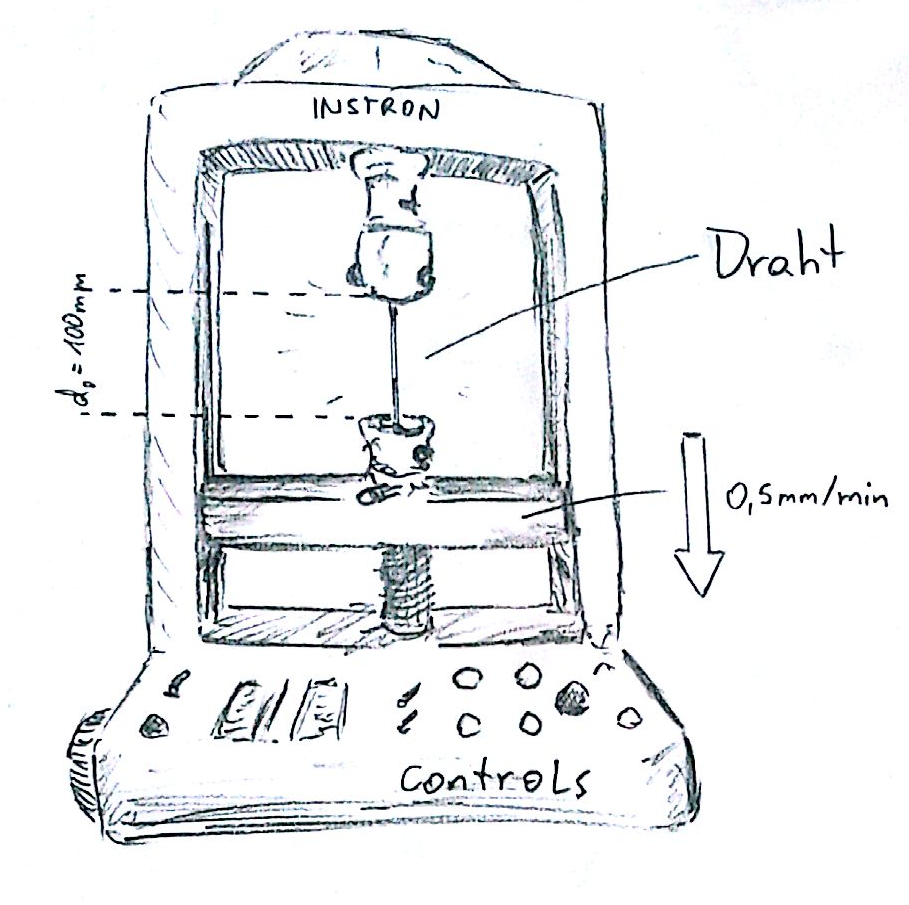
\includegraphics[scale=0.23]{./figure/zugversuch_aufbau.png}
	\caption{Skizze Versuchsaufbau}
	\label{fig:elastizitaet}
\end{figure}
\noindent
Die untere Klemme sitzt auf einem beweglichen Rahmen, der nach Beginn des Versuches mit 0.5 mm/min nach unten fährt. Dabei sendet die Kraftmesszelle im oberen Teil der Zugmaschine eine Spannung, proportional zur Kraft, die auf den Draht wirkt, an die Verstärkereinheit und über einen A/D-Wandler in den PC zur Aufzeichnung.\\
Das Signal wird in $[V]$ aufgezeichnet.\\
Daher muss die Datenausgabe vor Versuchsbeginn kalibriert werden:\\
Es werden 2 kg der Eichgewichte an der obere Klemme angebracht, und der Verstärker wird, mit Hilfe des Voltmeters) so eingestellt, dass 40mV ausgegeben werden:\\
$0.04 V \equiv 2 kg * 9.81 m/s^2 $\\
\\
Damit ergibt sich ein Umrechnungsfaktor von $1V \equiv 490,5 N $.\\
Schließlich muss die gemessene Kraft in Spannung umgerechnet werden durch $\sigma = \frac{F}{q}$, wobei q der Querschnitt des Drahtes ist.\\
Die aufgezeichnete Zeit wird durch\\
$ \epsilon = \frac{v*t}{L_{0}} $\\
in die Dehnung $\epsilon$ konvertiert, wobei die Geschwindigkeit des Zugrahmens\\
 $v = 0.5 mm/min$ und die Ausgangslänge $ L_{0} = (100 \pm 0.1) mm $.\\
\\
Die so gewonnenen Daten werden in einem Diagramm Spannung gegen Dehnung aufgetragen \ref{fig:orig_Vs_plot}.\\
Es wird ein linearer Anstieg im Elastizitätsbereich erwartet, dessen Steigung im linearen Fit direkt den E-Modul ergibt.\\

\begin{figure}[H]
\begin{tikzpicture}
    \pgfplotsset{width=7.4cm,
	}
    \begin{axis}[
    	xlabel={t(s)},
    	ylabel={mV}]
	\addplot [no marks,red]file{./data/ZugversuchBraun_Kurz2_edited.lvm};
    \end{axis}

    \end{tikzpicture}
    	\caption{Plot der Rohdaten aus der Messung}
	\label{fig:orig_Vs_plot}
\end{figure}

%"Für eine genauere Anleitung zur Versuchdurchführung siehe www....anfpra/pw3 %%%% ????
%\ref{fig:orig_Vs_plot}

\subsection{Messdaten und Ergebnisse}
Dicke des Aluminium-Drahtes [mm]:\\
$(1,98\pm 0.01)$mm\\
\\
(gemessen an 5 Stellen, gleichmäßig verteilt:
1.98
1.98
1.98
1.99
1.98\\
die Standardabw. des Mittelwerts ist trotz Student-t-Korrektur kleiner als die Auflösung des Messgerätes)\\
\\
Die folgenden Werte wurden direkt von QTi-Plot errechnet, und sinnvoll gerundet, durch die linearen Regressionen welche als rote Linien in Abbildung \ref{fig:draht_druck_dehnung_linreg} zu sehen sind.\\
Erste Steigung:\\
A = (13710 $\pm$ 230)N/$mm^2$\\
B = (-31.13 $\pm$ 0.78)N/$mm^2$\\
Zweite Steigung:\\
A = (55390 $\pm$ 480)N/$mm^2$\\
B = (-792.9$\pm$ 7.0) N/$mm^2$\\

%Voltmeter am Verstärker pendelt zwischen 9.98mV ohne Gewicht. Mit 2kg Last bei $(40 \pm 0.1)$mV. 

\section{Diskussion}
Ergibt eine Dicke von \textbf{$(1.99 \pm 0.01)mm$}. Die Unsicherheit ergibt sich aus der Ungenauigkeit des Messinstruments.
\begin{figure}[H]
	\centering
  	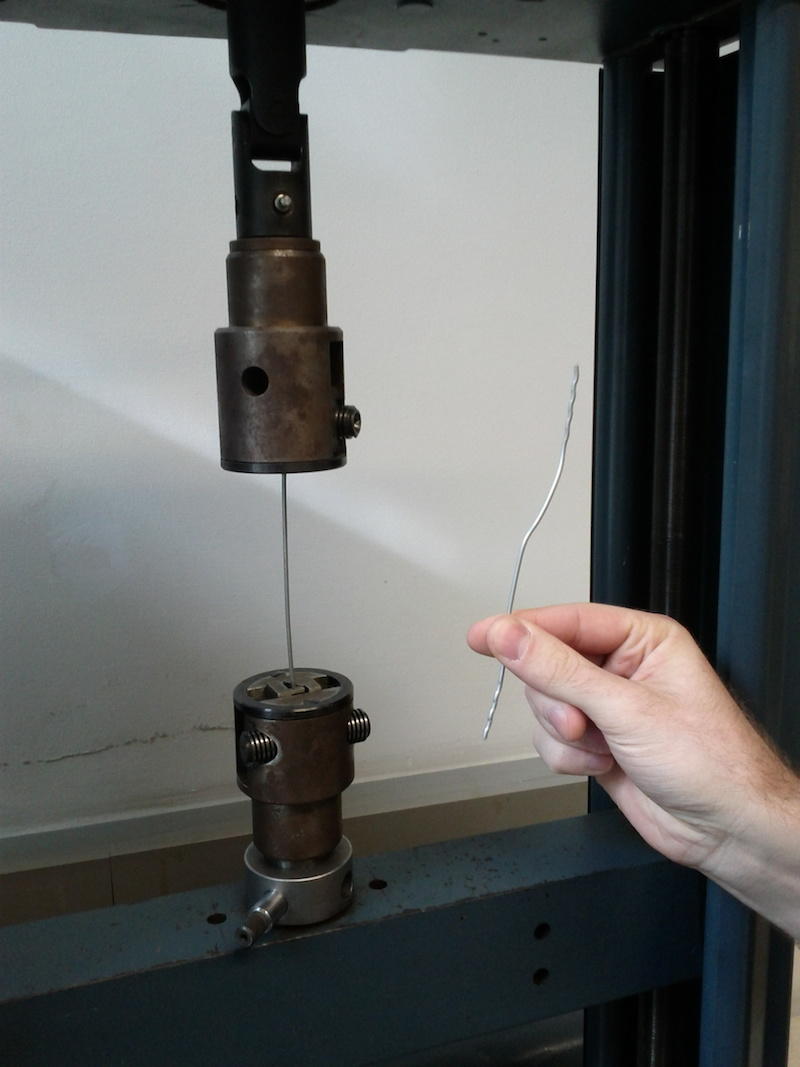
\includegraphics[scale=0.25]{./figure/zugversuch_fail.jpg}
	\caption{Korrekte Einspannung der Probe und Fehlversuch}
	\label{fig:draht_fehlversuch}
\end{figure}
\noindent
Da der erste Wert für $E_{Al}$ mit ($13710 \pm 230$)N/$mm^2$ deutlich niedriger ist, als der zweite, scheint die Probe verbogen gewesen zu sein und wir verwenden nur die zweite Steigung: 
$$E_{Al}=(55390 \pm 480)N/mm^2$$ 
ist noch weit entfernt vom Literaturwert $70000 N/mm^2$. Die Differenz könnte sich aus dem Abrutschenden des Drahtes aus der Halterung ergeben. Diese war möglicherweise bereits ausgebrochen und spröde. \\
Die Art der Einspannung, in der der zu untersuchende Draht sehr fest eingeklemmt werden muss, um nicht zu verrutschen, erzeugt auch eine Verformung, die das Messergebnis beeinflusst. Da relativ große Kräfte auf das Aluminium wirken, die jedoch im Idealfall nur auf eine Achse wirken sollten, ist die Genauigkeit dieser Methode, zumindest bei einem so dünnen Draht, nicht besonders hoch.\\
Das Experiment musste wiederholt werden, da beim ersten Versuch bereits die Probe durch Fehlbedienung, aufgrund der eben großen Kräfte sofort, verformt wurde (Ergebnisse wurden nicht berücksichtigt, siehe Probe Abbildung \ref{fig:draht_fehlversuch}).\\
Der erwartete Verlauf der Spannungs-Dehnungskurve ist dennoch, trotz der Ungenauigkeit, in \ref{fig:draht_druck_dehnung_linreg} gut zu erkennen.

\begin{figure}[H]
	\centering
  	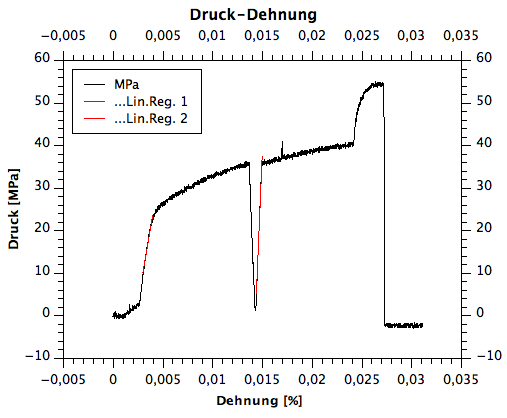
\includegraphics[scale=0.4]{./figure/druck_dehnung_linreg.png}
	\caption{Druck-Dehnungs Diagramm mit Fitting}
	\label{fig:draht_druck_dehnung_linreg}
\end{figure}

\section{Torsionspendel}
In diesem Teil von PW3 soll nun der Torsionsmodul G von Aluminium bestimmt werden. Aus diesem und dem in Kapitel 2 ermittelten Elastizitätsmodul E kann schließlich die Poissonzahl $\nu $ berechnet werden.\\

\begin{figure}[H]
	\centering
  	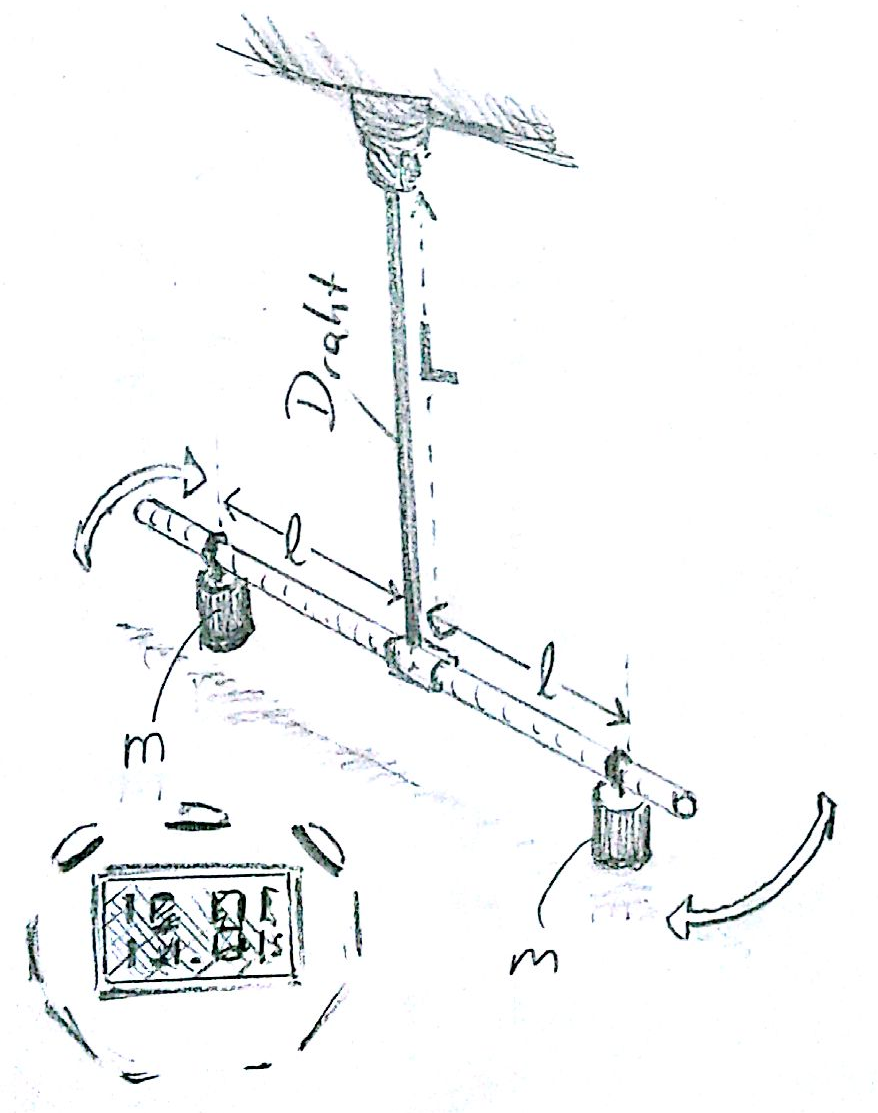
\includegraphics[scale=0.25]{./figure/torsionspendel_aufbau.png}
	\caption{Torsionspendel mit Massen}
	\label{fig:torsion}
\end{figure}

\subsection{Versuchsaufbau und \\-durchführung}
Equipment:
\begin{itemize}
	\item Ein Torsionspendel, bestehend aus einer Querstange, montiert an einem Aluminiumdraht
	\item Ein Satz Gewichte (je 2 gleiche)
	\item Eine Mikrometerschraube
	\item Ein Maßband
	\item Eine Stoppuhr
	\item Eine Waage
\end{itemize}
% !!!! bitte markennahmen, evtl auflösung/genauigkeit einfügen
Das Pendel wird aufgebaut, wie in \ref{fig:torsion}.\\
% !!!!!! skizze 3.1 einfügen... zeichnung - torsionspendel
2 gleiche Massen werden in gleichem Abstand l von der Mitte befestigt. Anschließend wird das Pendel derartig in Bewegung versetzt, dass die Querstange in der Ebene um ihre Ruhelage, also normal zum Aluminiumdraht, oszilliert. Der Draht erfährt also eine Scherung.\\
Es ist darauf zu achten, dass die Bewegung möglichst gleichmäßig und rund läuft. Eine nahezu saubere Torsion des Drahtes, ohne Verzerrungen, ist in dieser Art der Durchführung (von Hand) kaum möglich, einige Übungsläufe vor der ersten Messung können jedoch eindeutige Verbesserungen der Schwingung erwirken.\\
Mit der Stoppuhr wird die Dauer mehrerer Schwingungsperioden gemessen. Die Messung mehrerer Perioden bewirkt, dass der einigermaßen konstante Fehler durch die Ungenauigkeit beim Messen von Hand, geteilt wird und sein Einfluss auf einen einzelnen Durchgang damit wesentlich verringert wird.\\
Außerdem sollte beim Nulldurchgang, also dem Moment größter kinetischer Energie des Pendels gemessen werden. Eine Markierung des Nulldurchgangs unter dem ruhenden Pendel kann auch helfen, die Messung zu verbessern.\\
Der Torsionsmodul berechnet sich durch\\
$$G = \frac{2LD}{\pi r^4}$$
wobei L die Länge des Drahtes und D die Winkelrichtgröße ist.\\
Diese lässt sich aus dem Steiner'schen Satz durch Elimination mit 2 Messungen mit verschiedenem Abstand l (Entfernung der Massen vom Mittelpunkt) und damit 2 verschiedenen Periodendauern T ausdrücken:\\
$$ D=8\pi ^2 m* \frac{l_1^2-l_2^2}{T_1^2-T_2^2}$$
Aus beiden Gleichungen wird also G berechnet.\\
Zuletzt wird die Poissonzahl $\nu$, die das Verhältnis zwischen Änderung der Länge und des Durchmessers eines Festkörpers unter Spannung beschreibt, errechnet durch:\\
$$ \nu = \frac{E}{2G}-1$$

\subsection{Messdaten und Ergebnisse}


%Die Genauigkeit bei der Messung von Gewicht ist mit ($\pm 0.1$g) von der Waage und mit ($\pm 1mm$) bei dem Maßband vorgegeben.\\
%Messwerte $T_x$ für Messungen x $\in\{1,2,3,4\}$:\\

$T_1, T_2$: 10 Messungen zu je 10 Perioden
$T_3, T_4$:   5 Messungen zu je 20 Perioden
\begin{figure}[H]
	\centering
	\pgfplotstabletypeset[
			columns={T1,T2,T3,T4},
			col sep=tab,
			columns/T1/.style={column name=$T_1[s]$},
			columns/T2/.style={column name=$T_2[s]$},
			columns/T3/.style={column name=$T_3[s]$},
			columns/T4/.style={column name=$T_4[s]$},
			every head row/.style={before row=\hline,after row=\hline\hline},
			every last row/.style={after row=\hline},
			every first column/.style={
								column type/.add={|}{}
							        },
			every last column/.style={
								column type/.add={}{|}
								}
			]{./data/torsionspendel.dat}
	\caption{Periodendauer (0...keine Messung)}
	\label{fig:torsion_mw}
\end{figure}
\noindent
$L_{Draht} = (64.6 \pm 0.1)$cm\\
$r_{Draht} = (2.99 \pm 0.01)$ mm\\

\begin{itemize}
	\item Messreihe 1:\\
	Masse $m$: $\frac{1}{2}*(494.2 \pm 0.1$)g\\
	$l_1$ =   ($23.9 \pm 0.1)$ cm\\
	$T_1$ = ($1.30 \pm 0.02)$ s\\
	$l_2$  =  ($27.9 \pm 0.1$) cm\\
	$T_2$ = ($1.41 \pm 0.01$) s\\
	$$ G_1 = ( 27.91\pm 6.0)GPa$$\\
	
	%Fehler rechnen
	
	\item Messreihe 2:\\
	Masse $m$: $\frac{1}{2}*(729.7 \pm 0.1$)g\\
	$l_1$ =   ($34.9 \pm 0.1)$ cm\\
	$T_1$ = ($1.85 \pm 0.01)$ s\\
	$l_2$  =  ($47.9 \pm 0.1$) cm\\
	$T_2$ = ($2.44 \pm 0.01$) s\\
	$$ G_2 = (25.4 \pm 1.1 )GPa$$\\
\end{itemize}

\subsection{Diskussion}
Beide gemessenen Werte $G_1$ und $G_2$ für den Schubmodul von Aluminium stimmen mit dem Literaturwert von 25.5GPa überein.\\
Dabei ist der Wert aus der 2. Messreihe bedeutend genauer (also mit einer wesentlich kleineren Unsicherheit behaftet) und im Mittelwert sehr nahe am Literaturwert.
Einen sicherlich großen Einfluss auf diesen Unterschied der beiden Messungen, haben sicherlich die verschiedenen Versuchsdurchführungen:\\
Wie in \ref{fig:torsion_mw} ersichtlich, wurde die Periodendauer im ersten Versuch jeweils 10 mal für $T_1$ sowie $T_2$ gemessen, im zweiten Versuch nur 5 mal. Dafür wurden in Messreihe 1 jeweils nur 10 Schwingungen gemessen, um auf eine Periode rückzurechnen, in Messreihe 2 jedoch 20.\\
Da die Zeitmessung von Hand, mit der Stoppuhr durchgeführt wurde, hilft diese Vorgehensweise, die Fehler durch menschliche Ungenauigkeiten, zu verkleinern (eben um den Faktor $\frac{1}{10}$ oder $\frac{1}{20}$.)\\
Da jedoch (mit einer Ausnahme) der Standarderror-of-the-mean bei allen Messungen kleiner als die Auflösung der Stoppuhr war, ist die Hauptursache für den Unterschied in der Genauigkeit sicherlich woanders zu suchen.\\
Die 2. Messreihe unterscheidet sich auch durch die Wahl der Massen und der ihrer Abstände l von der ersten:\\
Diese wurden alle deutlich größer gewählt, als ihre Pendants in der ersten Messreihe. Das führt zu deutlich langsameren Periodendauern, die sowohl einfacher zu messen sind, als auch das System ruhiger schwingen lassen.\\
Der Aufbau und die verwendeten Verhältnisse haben in diesem Experiment eine ebenmäßige Schwingung des Pendels fast unmöglich gemacht (Anregung per Hand). Auch das war in der 2. Messreihe näher am Ideal.\\
\\
\textbf{Poissonzahl $\nu_{Al}$}\\
Zuletzt soll noch aus dem Elastizitätsmodul $E_{Al}$ für Aluminium aus \ref{Elastizität} und dem ermittelten Schubmodul $G_{Al}$ die Poissonzahl errechnet werden:\\
\\
$\nu_{Al} = (0.090 \pm 0.049)$\\
\\
Die doch sehr große Abweichung vom Literaturwert ($\nu_{Al}=0.34$) erklärt sich einfach durch das eher ungenau Ergebnis für $E_{Al}$. Ersetzt man dieses durch seinen Literaturwert, stimmt auch die Poissonzahl (in den Grenzen der Unsicherheit) überein.


%%%% FAHRRADPENDEL %%%%%


\section{Pendel}
\begin{figure}[H]
	\centering
  	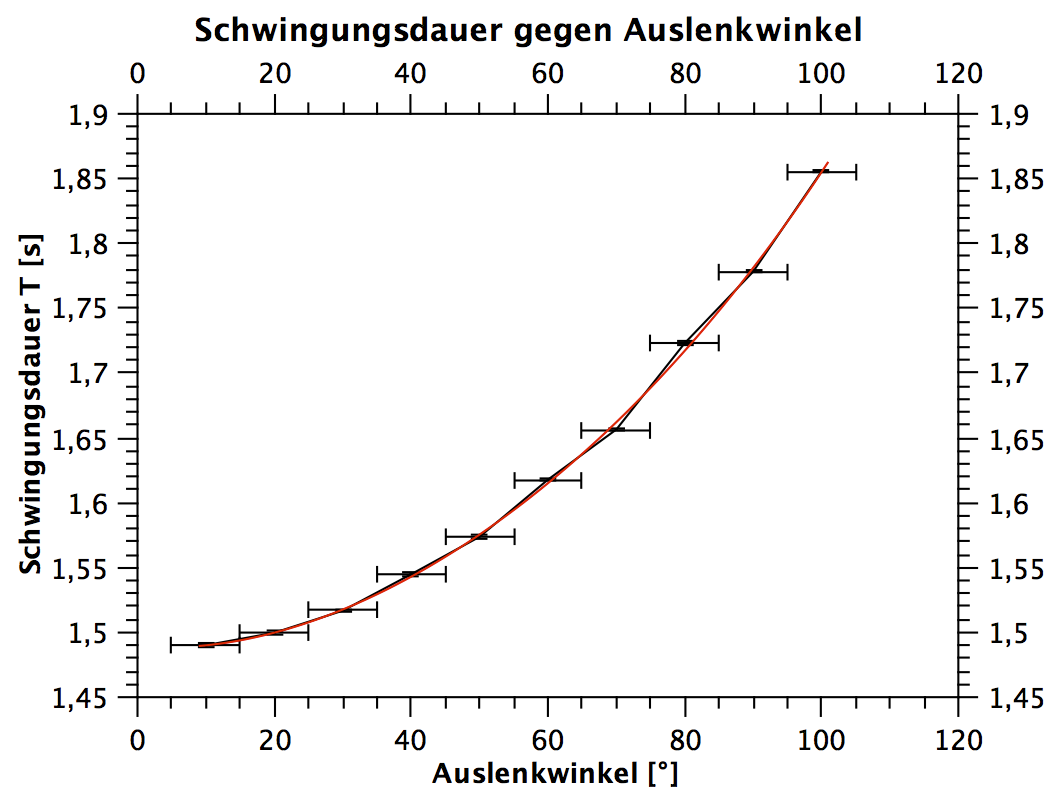
\includegraphics[scale=0.45]{./figure/speichenrad_fit_error.png}
	\caption{Speichenradmessungen mit Fehlerbalken und Polynomiellem Fitting}
	\label{fig:rad_fit}
\end{figure}
\noindent
In diesem Versuch soll das gesamte , sowie die einzelnen Teilträgheitsmomente eines physikalischen Pendels, bestehend aus einem Rad und einem daran montierten Zylinder, ermittelt werden.\\
Dazu wird der Steiner'sche Satz benutzt, der das Trägheitsmoment eines Körpers für seine Drehung um den Schwerpunkt mit dem Trägheitsmoment J um eine parallele Achse verbindet (Abstand d zwischen den Achsen).\\
$$ J = J_{S} + m_{ges}d^2 $$

\subsection{Versuchsaufbau und \\-durchführung}

\begin{itemize}
	\item Ein Rad mit Aufhängung
	\item Ein Metallzylinder
	\item Ein Maßband (Auflösung $1 mm$)
	\item Eine Schiebelehre (Aufl. $0.05mm$)
	\item CASSY - Sensorsystem
\end{itemize}

\begin{figure}[H]
	\centering
  	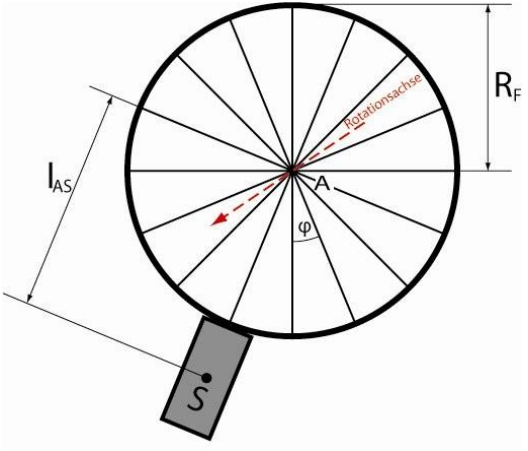
\includegraphics[scale=0.4]{./figure/speichenrad.png}
	\caption{Speichenrad mit Zylindermasse}
	\label{fig:rad}
\end{figure}
\noindent
Das hier untersuchte Pendel besteht aus einem Speichenrad, durch dessen Mittelpunkt die Drehachse geht, und einem an der Außenseite befestigten Metallzylinder \ref{fig:rad}.\\
Das gesamte Trägheitsmoment des Systems ist die Summe der einzelnen, von Rad und Zylinder. Da das Trägheitsmoment des Rades aufgrund seiner inhomogenen Masseverteilung und Form jedoch mathematisch nicht zu erhalten ist, errechnet man aus der Periodendauer der Schwingung im Grenzfall des Auslenkwinkels $\varphi_{0} \rightarrow 0$ das gesamte Trägheitmoment und erhält so gemeinsam mit dem des Zylinders schließlich auch das des Rades:\\

$$ J = J_{Z} + J_{Rad} = D*(\frac{T_{0}}{2\pi})^2$$

Die Winkelrichtgröße D:\\

$$D=m_{z}*g*l_{AS}$$\\

Das Trägheitsmoment des Zylinders:\\

$$J_{Z}=m_{Z}(\frac{1}{4}r_{Z}^2 + \frac{1}{12}h_{Z}^2+l_{AS}^2)$$

, wobei $l_{AS}$ der Abstand zwischen Drehachse und Schwerpunkt ist.\\
Die Periodendauer $T_{0}$ erhält man, indem die Periodendauern verschiedener Auslenkwinkel $\varphi$ gemessen werden und aus den Einzelwerten mittels Polynom-Fit auf die Schwingungsdauer $T(\varphi_{0})$ extrapoliert werden kann.\\
Dazu wird in Abständen von $10^{\circ}$, beginnend mit $100^{\circ}$, die Schwingungsdauer computergestützt mit einem Sensor-CASSY gemessen.




\subsection{Messdaten und Ergebnisse}
\begin{itemize}
	\item Zylinder:\\
	$m_{Z}= (938,5 \pm 0.1)g$\\
	$h_{Z} = (107.60 \pm 0.02)mm$\\
	$r_{Z}=(35.28 \pm 0.02)mm$\\
	
	\item Achsenabstand\\
	$l_{AS}=(388\pm 1)mm$\\
	
	\item Periodendauer ($\varphi_{0}$)\\
	$T_{0}= (1.490 \pm 0.001)s$\\
	
\end{itemize}


$$J_{Z}= (0.142 \pm 0.001)kg*m^2$$
$$J_{Ges}= (0.201\pm 0.053)kg*m^2$$
$$J_{Rad}= (0.0585 \pm 0.052)kg*m^2$$


\subsection{Diskussion}



\section{Quellen}
Formeln und Abbildung Fahrradpendel:\\
\url{http://www.univie.ac.at/anfpra/neu1/pw/pw3/PW3.pdf}\\
\url{http://de.wikipedia.org/wiki/Schubmodul}\\
\\

\end{multicols}
\end{document}